\section{全量响应、预测与扩展结果}
\label{cr:results}
\subsection{封存快照与样本完成度}
本次证据截止为\EvidenceDate。完整训练和测试均经原档重审，未读取在途或原FAILED电学输出。四alias仅提供其原逻辑槽，来源含实际run、owner plan、case-freeze与输入/归档SHA。
快照内部分图件状态保留采集时的PENDING标签，未回写历史快照；后续完整机器、统计和逐图目视验收另见\sourcepath{data/delivery-root-acceptance.json}及两份visual-review记录。本文将采集时状态与事后验收证书分开引用。

\begin{table}[htbp]
\centering\small
\caption{完整主矩阵的样本与响应分配；同事件两位不独立翻倍。}
\label{cr:progress}
\begin{tabular}{lrrrr}
\toprule
集合 & 独立事件 & 配对响应 & 已验证 & 缺失\\
\midrule
训练0.18/0.35 $\mu$m & 32 & 64 & 64 & 0\\
域内0.25 $\mu$m & 16 & 32 & 32 & 0\\
外推0.45 $\mu$m & 16 & 32 & 32 & 0\\
\bottomrule
\end{tabular}

\end{table}
\subsection{匹配参考与预充修订的历史依据}
历史D1无粒子诊断中，固定理想参考留下约12.37~mV读出偏移；同一信号状态改用匹配中性参考后，差分从+2.454961~mV变为-9.915036~mV。该诊断说明参考会改变判据解释，不纳入R50主矩阵。原100~$\Omega$固定事件的3~ns预充误差为-13.297362~$\mu$V，超过10~$\mu$V原门槛；独立50~$\Omega$ probe对应误差为-4.731204~$\mu$V，随后才建立独立统一主版本。

\begin{figure}[htbp]
\centering
\includegraphics[width=.85\textwidth]{d1-reference-comparison.pdf}
\caption{历史D1参考诊断，仅用于解释方法演进；原始分类不追溯替换。}
\label{cr:d1}
\end{figure}

\begin{figure}[htbp]
\centering
\includegraphics[width=.85\textwidth]{r50-precharge.pdf}
\caption{历史100~$\Omega$失败与独立50~$\Omega$ probe。两者均不作为新的R50主事件。}
\label{cr:precharge}
\end{figure}
\subsection{完整128响应与三阈值统计}
在5~mV主阈值下，128个响应中96项正确、20项判据误读、8项临界、4项数值不确定，失败和缺失各为0与0项。
每个尺寸/粒子/方向/位值分层的预定N保持4，零次明确误读不能推出总体风险为零。表中有效分类已传播近界和细化跨界不确定性，原分类另见完整响应CSV。

\begin{table}[htbp]
\centering\small
\caption{完整128响应在三阈值下的有效状态；失败与缺失不计为正确。}
\label{cr:thresholds}
\begin{tabular}{rrrrrrr}
\toprule
阈值/mV & 正确 & 判据误读 & 临界 & 数值不确定 & 失败 & 缺失\\
\midrule
2.5 & 96 & 27 & 4 & 1 & 0 & 0\\
5 & 96 & 20 & 8 & 4 & 0 & 0\\
10 & 96 & 5 & 26 & 1 & 0 & 0\\
\bottomrule
\end{tabular}

\end{table}

\begin{table}[htbp]
\centering\footnotesize
\caption{按栅长、粒子、位值列出的连续响应范围；每行合并两方向共8响应，未额外增加独立样本。}
\label{cr:ranges}
\begin{tabular}{lclrrr}
\toprule
$L$/\,$\mu$m & 粒子 & 位 & $\Delta Q$/fC & $\Delta M$/mV & $M$/mV\\
\midrule
0.18 & $\alpha$ & 0 & -4.821至-3.560 & -45.514至-33.619 & 71.116至83.011\\
0.18 & $\alpha$ & 1 & -5.412至-3.967 & 37.026至50.550 & -13.213至0.311\\
0.18 & 质子 & 0 & -0.402至-0.164 & -3.784至-1.545 & 39.041至41.281\\
0.18 & 质子 & 1 & -0.436至-0.181 & 1.685至4.066 & 33.270至35.651\\
0.25 & $\alpha$ & 0 & -4.701至-3.732 & -44.357至-35.148 & 72.537至81.746\\
0.25 & $\alpha$ & 1 & -5.166至-4.118 & 38.339至48.114 & -10.880至-1.105\\
0.25 & 质子 & 0 & -0.460至-0.239 & -4.317至-2.241 & 39.631至41.706\\
0.25 & 质子 & 1 & -0.496至-0.257 & 2.391至4.609 & 32.626至34.844\\
0.35 & $\alpha$ & 0 & -4.862至-4.081 & -45.601至-38.220 & 75.376至82.757\\
0.35 & $\alpha$ & 1 & -5.307至-4.459 & 41.259至49.125 & -12.119至-4.253\\
0.35 & 质子 & 0 & -0.456至-0.145 & -4.250至-1.354 & 38.510至41.406\\
0.35 & 质子 & 1 & -0.488至-0.155 & 1.435至4.509 & 32.496至35.571\\
0.45 & $\alpha$ & 0 & -4.834至-3.886 & -45.066至-36.161 & 73.090至81.994\\
0.45 & $\alpha$ & 1 & -5.249至-4.208 & 38.699至48.287 & -11.506至-1.918\\
0.45 & 质子 & 0 & -0.509至-0.229 & -4.716至-2.120 & 39.048至41.645\\
0.45 & 质子 & 1 & -0.544至-0.244 & 2.237至5.000 & 31.781至34.544\\
\bottomrule
\end{tabular}

\end{table}

\begin{figure}[htbp]
\centering
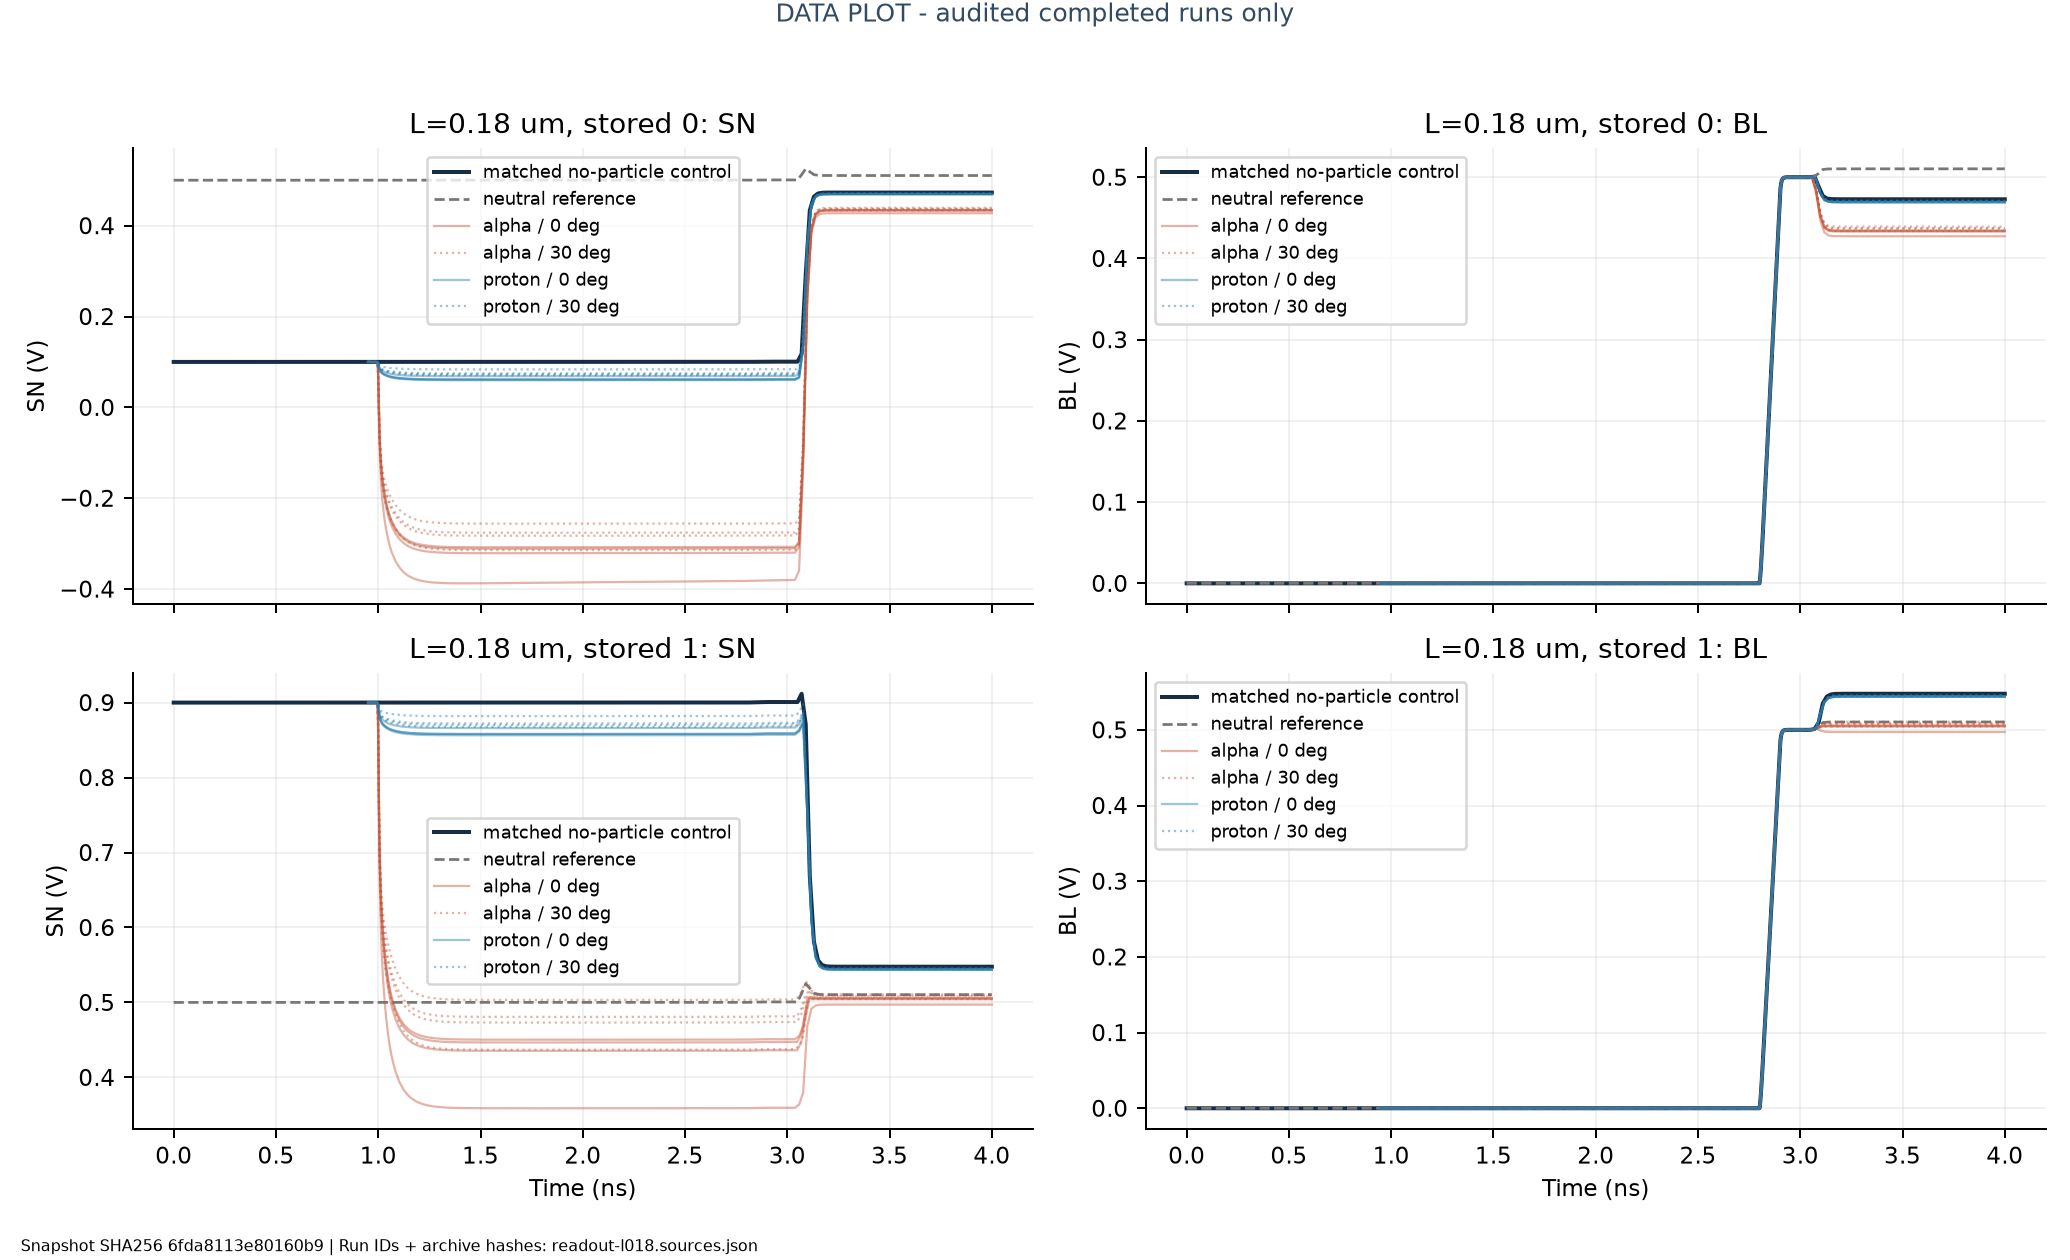
\includegraphics[width=.95\textwidth]{readout-l018.png}
\caption{0.18~$\mu$m的全部事件、同位control与neutral读出曲线；数据来自统一R50快照。}
\label{cr:readout}
\end{figure}

\begin{figure}[htbp]
\centering
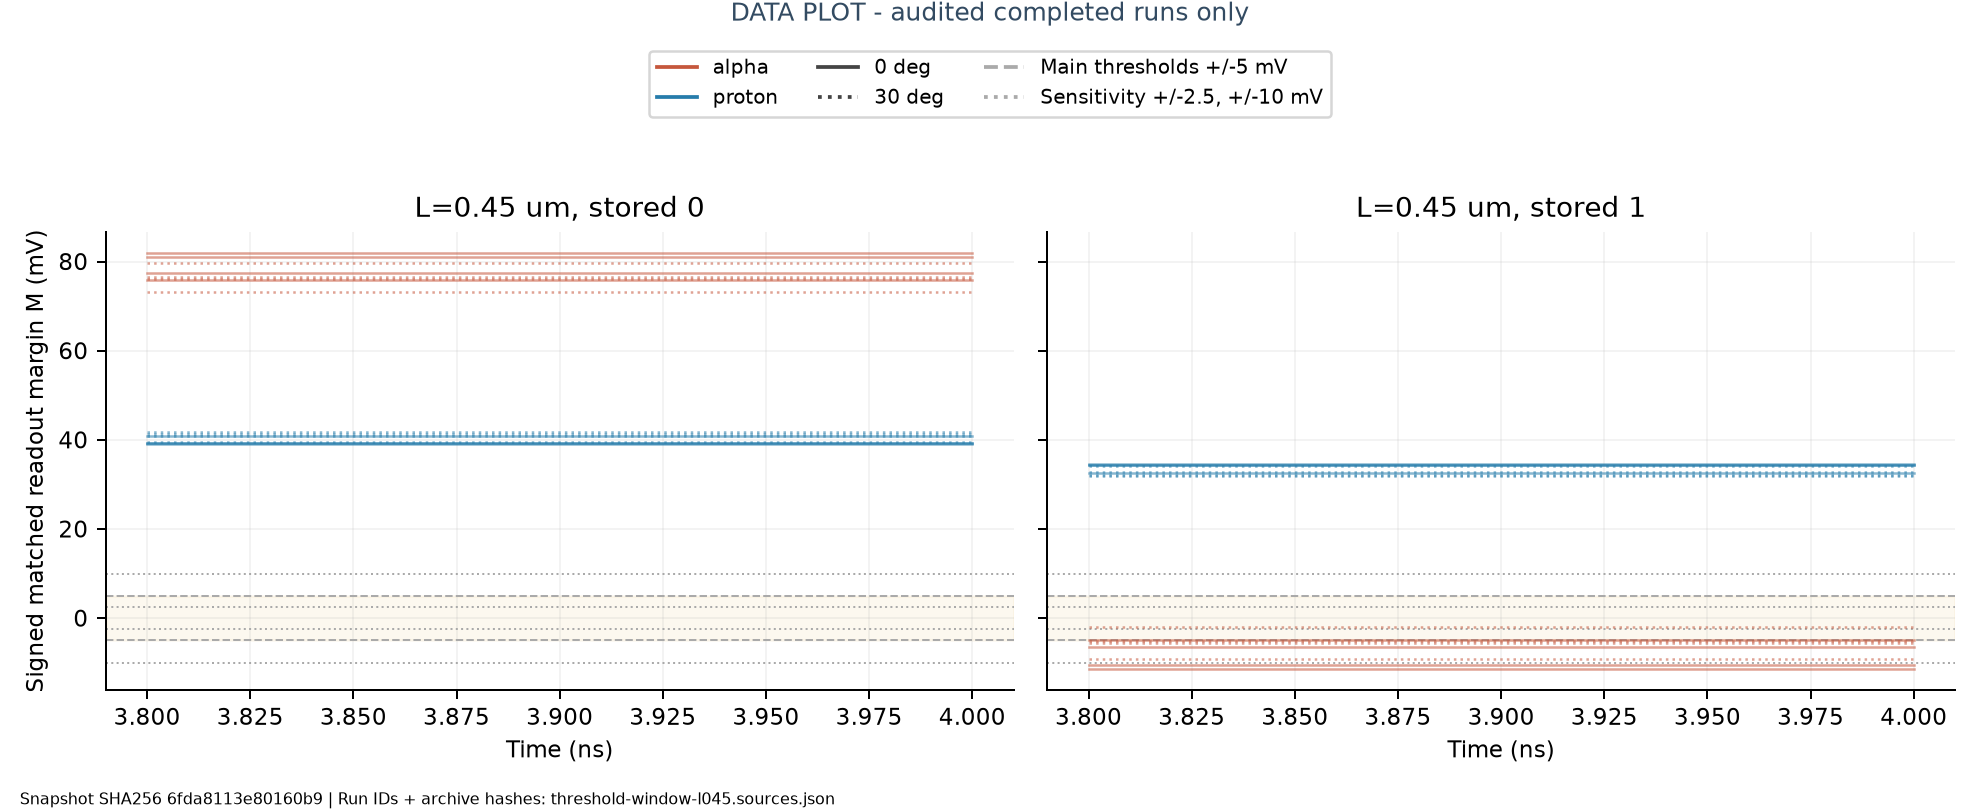
\includegraphics[width=.95\textwidth]{threshold-window-l045.png}
\caption{0.45~$\mu$m外推集合在3.8至4~ns的读出裕量窗口；线条和阈值均来自封存快照。}
\label{cr:window}
\end{figure}
\subsection{原冻结模型的独立留出与外推}
四模型由训练工况LOCO选择，冻结后不再调参。
\begin{table}[htbp]
\centering\small
\caption{八个物理工况折RMSE的算术平均；仅用于训练阶段模型选择。}
\label{cr:cv}
\begin{tabular}{llrrr}
\toprule
位 & 目标 & $\lambda$ & 岭回归RMSE & 均值基准RMSE\\
\midrule
0 & $\Delta Q$/fC & 0.1 & 0.102888 & 2.279967\\
0 & $\Delta M$/mV & 0.1 & 0.955160 & 21.458870\\
1 & $\Delta Q$/fC & 0.1 & 0.112903 & 2.515710\\
1 & $\Delta M$/mV & 0.1 & 1.012491 & 23.383861\\
\bottomrule
\end{tabular}

\end{table}
域内留出的存储0/1岭回归RMSE分别为0.088294/0.094644~fC（电荷）和0.798415/0.838043~mV（裕量损失）。尺寸外推的存储0/1岭回归RMSE分别为0.068049/0.067155~fC（电荷）和0.519434/0.504929~mV（裕量损失）。本次原r4评分与最终连续有效性评分逐项一致。
分类临界或跨界与连续量有效性分别处理；原r4首次评分的原字节副本与最终数值评分均附在证据包。

\begin{table}[htbp]
\centering\footnotesize
\caption{$\Delta Q$的固定预测误差，单位fC。每模型/位/集合计划16响应；缺失和无效显式报告。}
\label{cr:scoreq}
\begin{tabular}{lllrrrrrr}
\toprule
集合 & 位 & 模型 & $n$ & 缺失 & 无效 & MAE & RMSE & 最大误差\\
\midrule
留出 & 0 & 均值基准 & 16 & 0 & 0 & 1.942616 & 1.956036 & 2.416036\\
留出 & 0 & 岭回归 & 16 & 0 & 0 & 0.056607 & 0.088294 & 0.181592\\
留出 & 1 & 均值基准 & 16 & 0 & 0 & 2.140865 & 2.154850 & 2.651122\\
留出 & 1 & 岭回归 & 16 & 0 & 0 & 0.061766 & 0.094644 & 0.198945\\
外推 & 0 & 均值基准 & 16 & 0 & 0 & 2.011262 & 2.025386 & 2.548969\\
外推 & 0 & 岭回归 & 16 & 0 & 0 & 0.052826 & 0.068049 & 0.136393\\
外推 & 1 & 均值基准 & 16 & 0 & 0 & 2.183932 & 2.198297 & 2.733561\\
外推 & 1 & 岭回归 & 16 & 0 & 0 & 0.051740 & 0.067155 & 0.144228\\
\bottomrule
\end{tabular}

\end{table}

\begin{table}[htbp]
\centering\footnotesize
\caption{$\Delta M$的固定预测误差，单位mV。测试没有反向参与选模。}
\label{cr:scorem}
\begin{tabular}{lllrrrrrr}
\toprule
集合 & 位 & 模型 & $n$ & 缺失 & 无效 & MAE & RMSE & 最大误差\\
\midrule
留出 & 0 & 均值基准 & 16 & 0 & 0 & 18.320612 & 18.448022 & 22.860163\\
留出 & 0 & 岭回归 & 16 & 0 & 0 & 0.526964 & 0.798415 & 1.645649\\
留出 & 1 & 均值基准 & 16 & 0 & 0 & 19.936695 & 20.066626 & 24.741705\\
留出 & 1 & 岭回归 & 16 & 0 & 0 & 0.549768 & 0.838043 & 1.765441\\
外推 & 0 & 均值基准 & 16 & 0 & 0 & 18.742144 & 18.867683 & 23.569637\\
外推 & 0 & 岭回归 & 16 & 0 & 0 & 0.404964 & 0.519434 & 1.075289\\
外推 & 1 & 均值基准 & 16 & 0 & 0 & 20.091257 & 20.219896 & 24.915029\\
外推 & 1 & 岭回归 & 16 & 0 & 0 & 0.387723 & 0.504929 & 1.105078\\
\bottomrule
\end{tabular}

\end{table}

\begin{figure}[htbp]
\centering
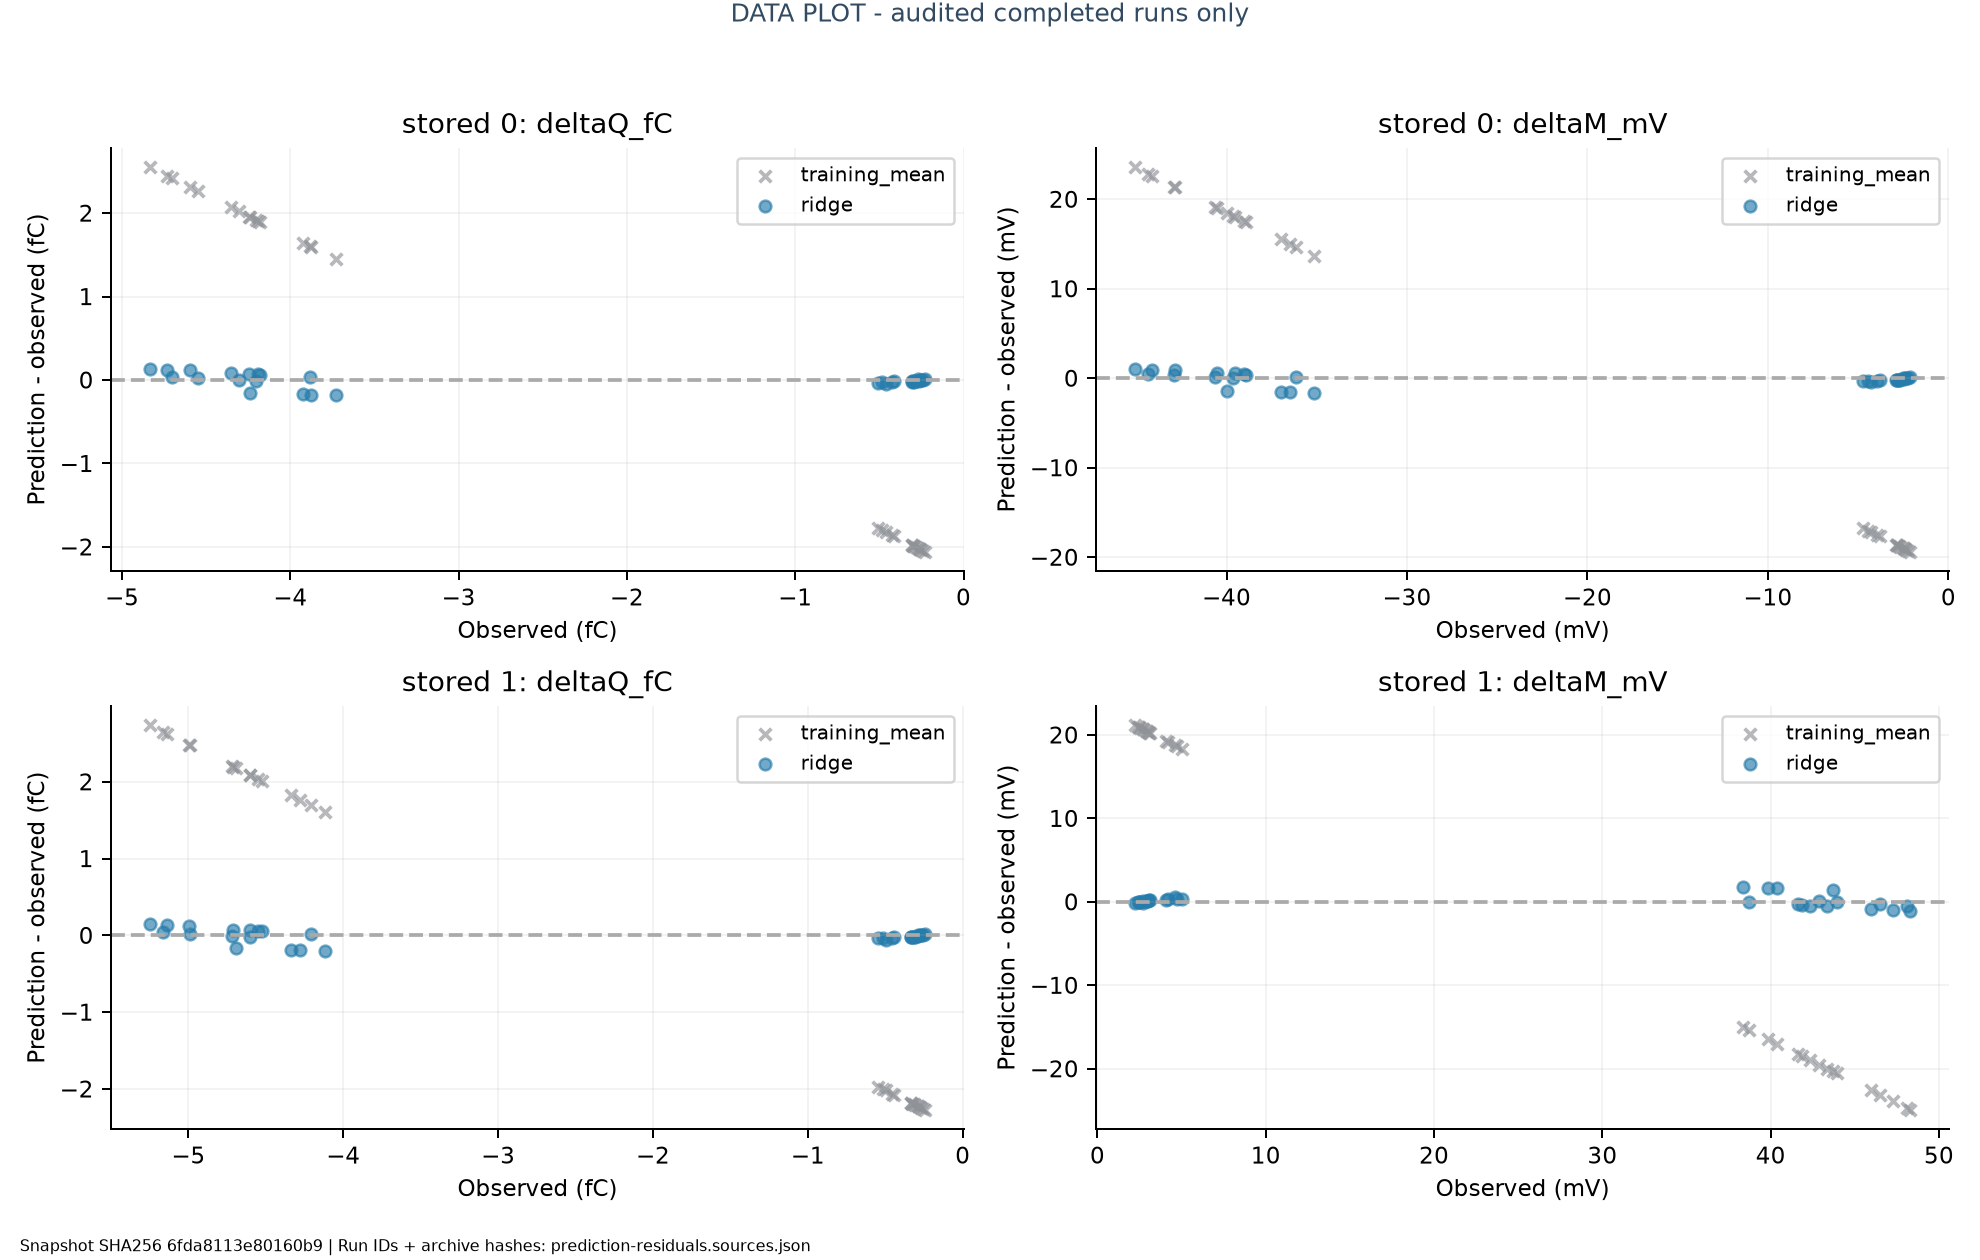
\includegraphics[width=.95\textwidth]{prediction-residuals.png}
\caption{冻结预测减去实际观测的留出/外推残差；训练均值与岭回归均保留。}
\label{cr:residuals}
\end{figure}
\subsection{氧化层敏感性}
在0.25~$\mu$m、垂直入射的固定alpha/质子首个事件上，4/6~nm厚度各建立独立0/1对照、中性参考和事件响应，共14个case。5~nm复用对应四个主响应；含原质子bit0的r3有效alias。每个新厚度实际重建网格，事件三文件字节保持一致。

\begin{table}[htbp]
\centering\footnotesize
\caption{相对于对应5~nm响应的氧化层变化；$\delta(\Delta Q)$和$\delta(\Delta M)$是新厚度减5~nm。}
\label{cr:oxide}
\begin{tabular}{llrrrr}
\toprule
粒子 & 位 & $t_{ox}$/nm & $\delta(\Delta Q)$/fC & $\delta(\Delta M)$/mV & $M$/mV\\
\midrule
$\alpha$ & 0 & 4 & -0.00240 & 0.06772 & 77.8443\\
$\alpha$ & 0 & 6 & -0.00578 & -0.11012 & 78.1679\\
$\alpha$ & 1 & 4 & -0.00464 & -0.06297 & -6.7275\\
$\alpha$ & 1 & 6 & -0.00484 & 0.11256 & -6.7559\\
质子 & 0 & 4 & -0.00022 & 0.00324 & 39.5380\\
质子 & 0 & 6 & -0.00028 & -0.00589 & 39.6928\\
质子 & 1 & 4 & -0.00022 & -0.00377 & 34.7574\\
质子 & 1 & 6 & -0.00027 & 0.00621 & 34.8945\\
\bottomrule
\end{tabular}

\end{table}

\begin{figure}[htbp]
\centering
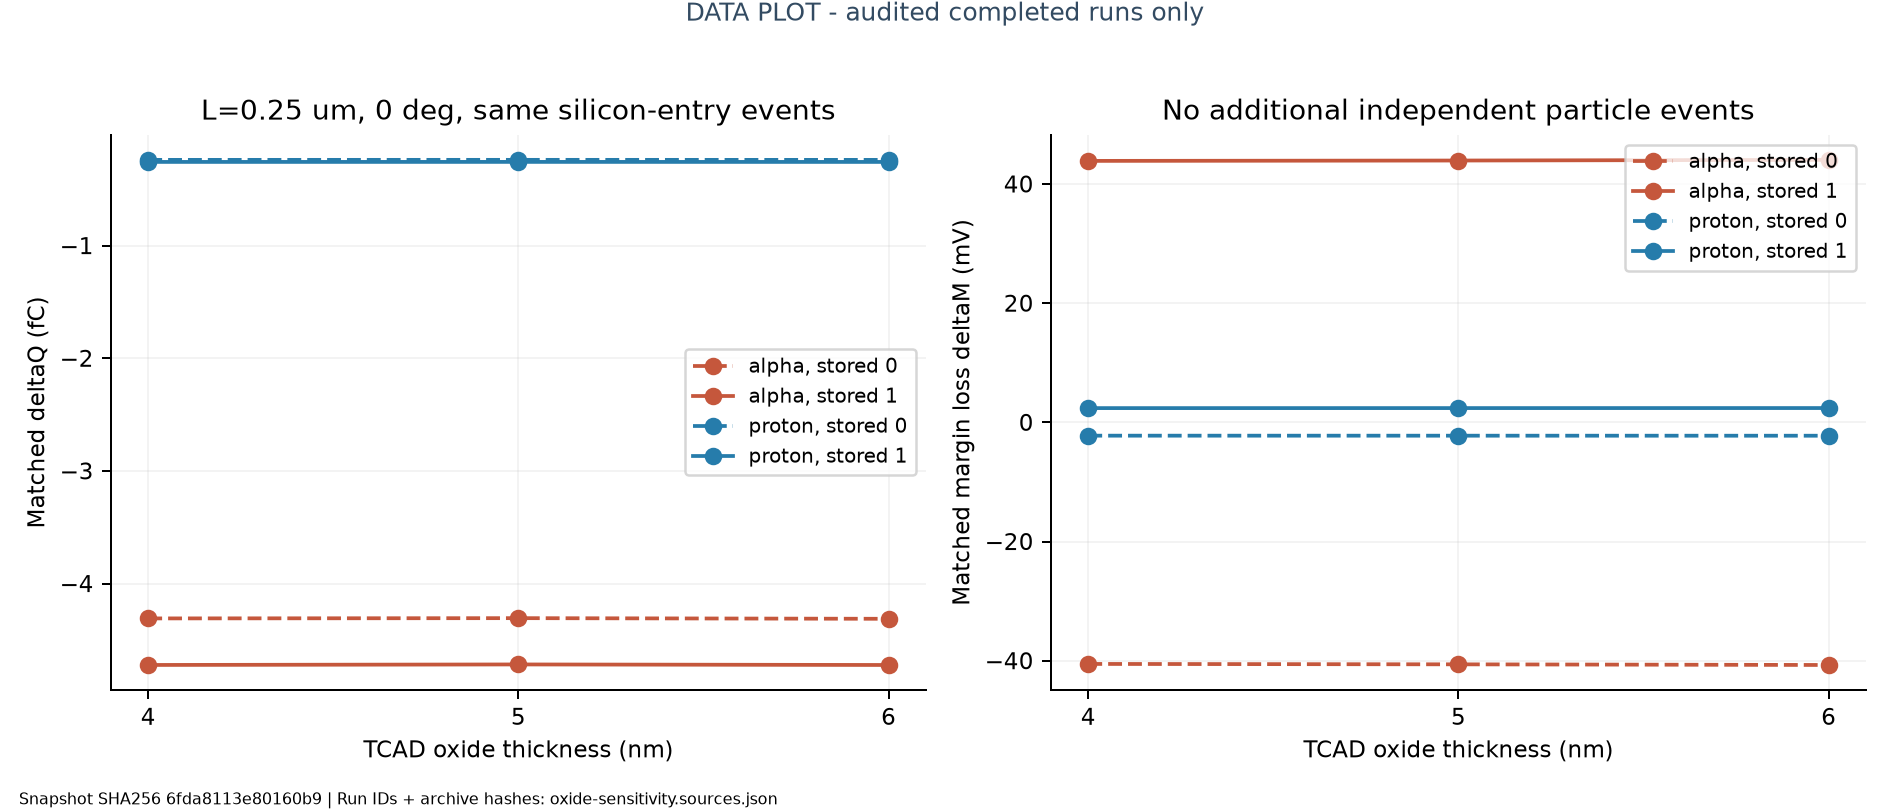
\includegraphics[width=.95\textwidth]{oxide-sensitivity.png}
\caption{4/5/6~nm在固定硅入口事件下的TCAD敏感性；不表示变化材料栈的Geant4输运。}
\label{cr:oxidefig}
\end{figure}
八个新事件响应相对于5~nm的最大绝对变化为0.112560497~mV（裕量损失）和约0.005783687~fC（电荷），分类保持。这些幅度小于预定验收容差0.5~mV和0.01~fC；容差不是统计误差条或已估计的分辨率。每个氧化层响应未再做独立细化和统计校准，故只报告固定入口事件下幅度较小的受控敏感性，不主张零效应、微小效应已可靠分辨或统计显著性。
\subsection{完整矩阵边界细化与原生图}
边界目标由完整128响应到$\pm2.5/5/10$~mV的最小距离排序选取，保持原规则和目标。每目标分别使用半步长与0.7网格的匹配control/neutral/event。四项连续比较均通过，但连续通过不代表类别稳定；5~mV跨界及未选近界响应继续保留不确定性。

\begin{table}[htbp]
\centering\footnotesize
\caption{四个边界比较。最大电压变化包含规定的两侧BL与派生读出量；容差0.5~mV和0.01~fC。}
\label{cr:boundary}
\begin{tabular}{llrrll}
\toprule
事件/位 & 变体 & 最大电压变化/mV & $|\delta\Delta Q|$/fC & 连续门槛 & 不确阈值/mV\\
\midrule
202610304/b1 & 半步长 & 0.032654 & 0.003490 & 通过 & 5\\
202610304/b1 & 0.7网格 & 0.005088 & 0.000009 & 通过 & 无\\
202610313/b1 & 半步长 & 0.025337 & 0.002709 & 通过 & 无\\
202610313/b1 & 0.7网格 & 0.005088 & 0.000006 & 通过 & 无\\
\bottomrule
\end{tabular}

\end{table}

\begin{table}[htbp]
\centering\small
\caption{128响应乘三阈值的384个状态。界外未细化不冒称全部网格独立。}
\label{cr:uncertainty}
\begin{tabular}{lr}
\toprule
阈值响应对状态 & 数量/384\\
\midrule
细化稳定 & 8\\
分类跨界 & 1\\
连续失败 & 0\\
近界待确认 & 5\\
界外未细化 & 370\\
\bottomrule
\end{tabular}

\end{table}

\begin{figure}[htbp]
\centering
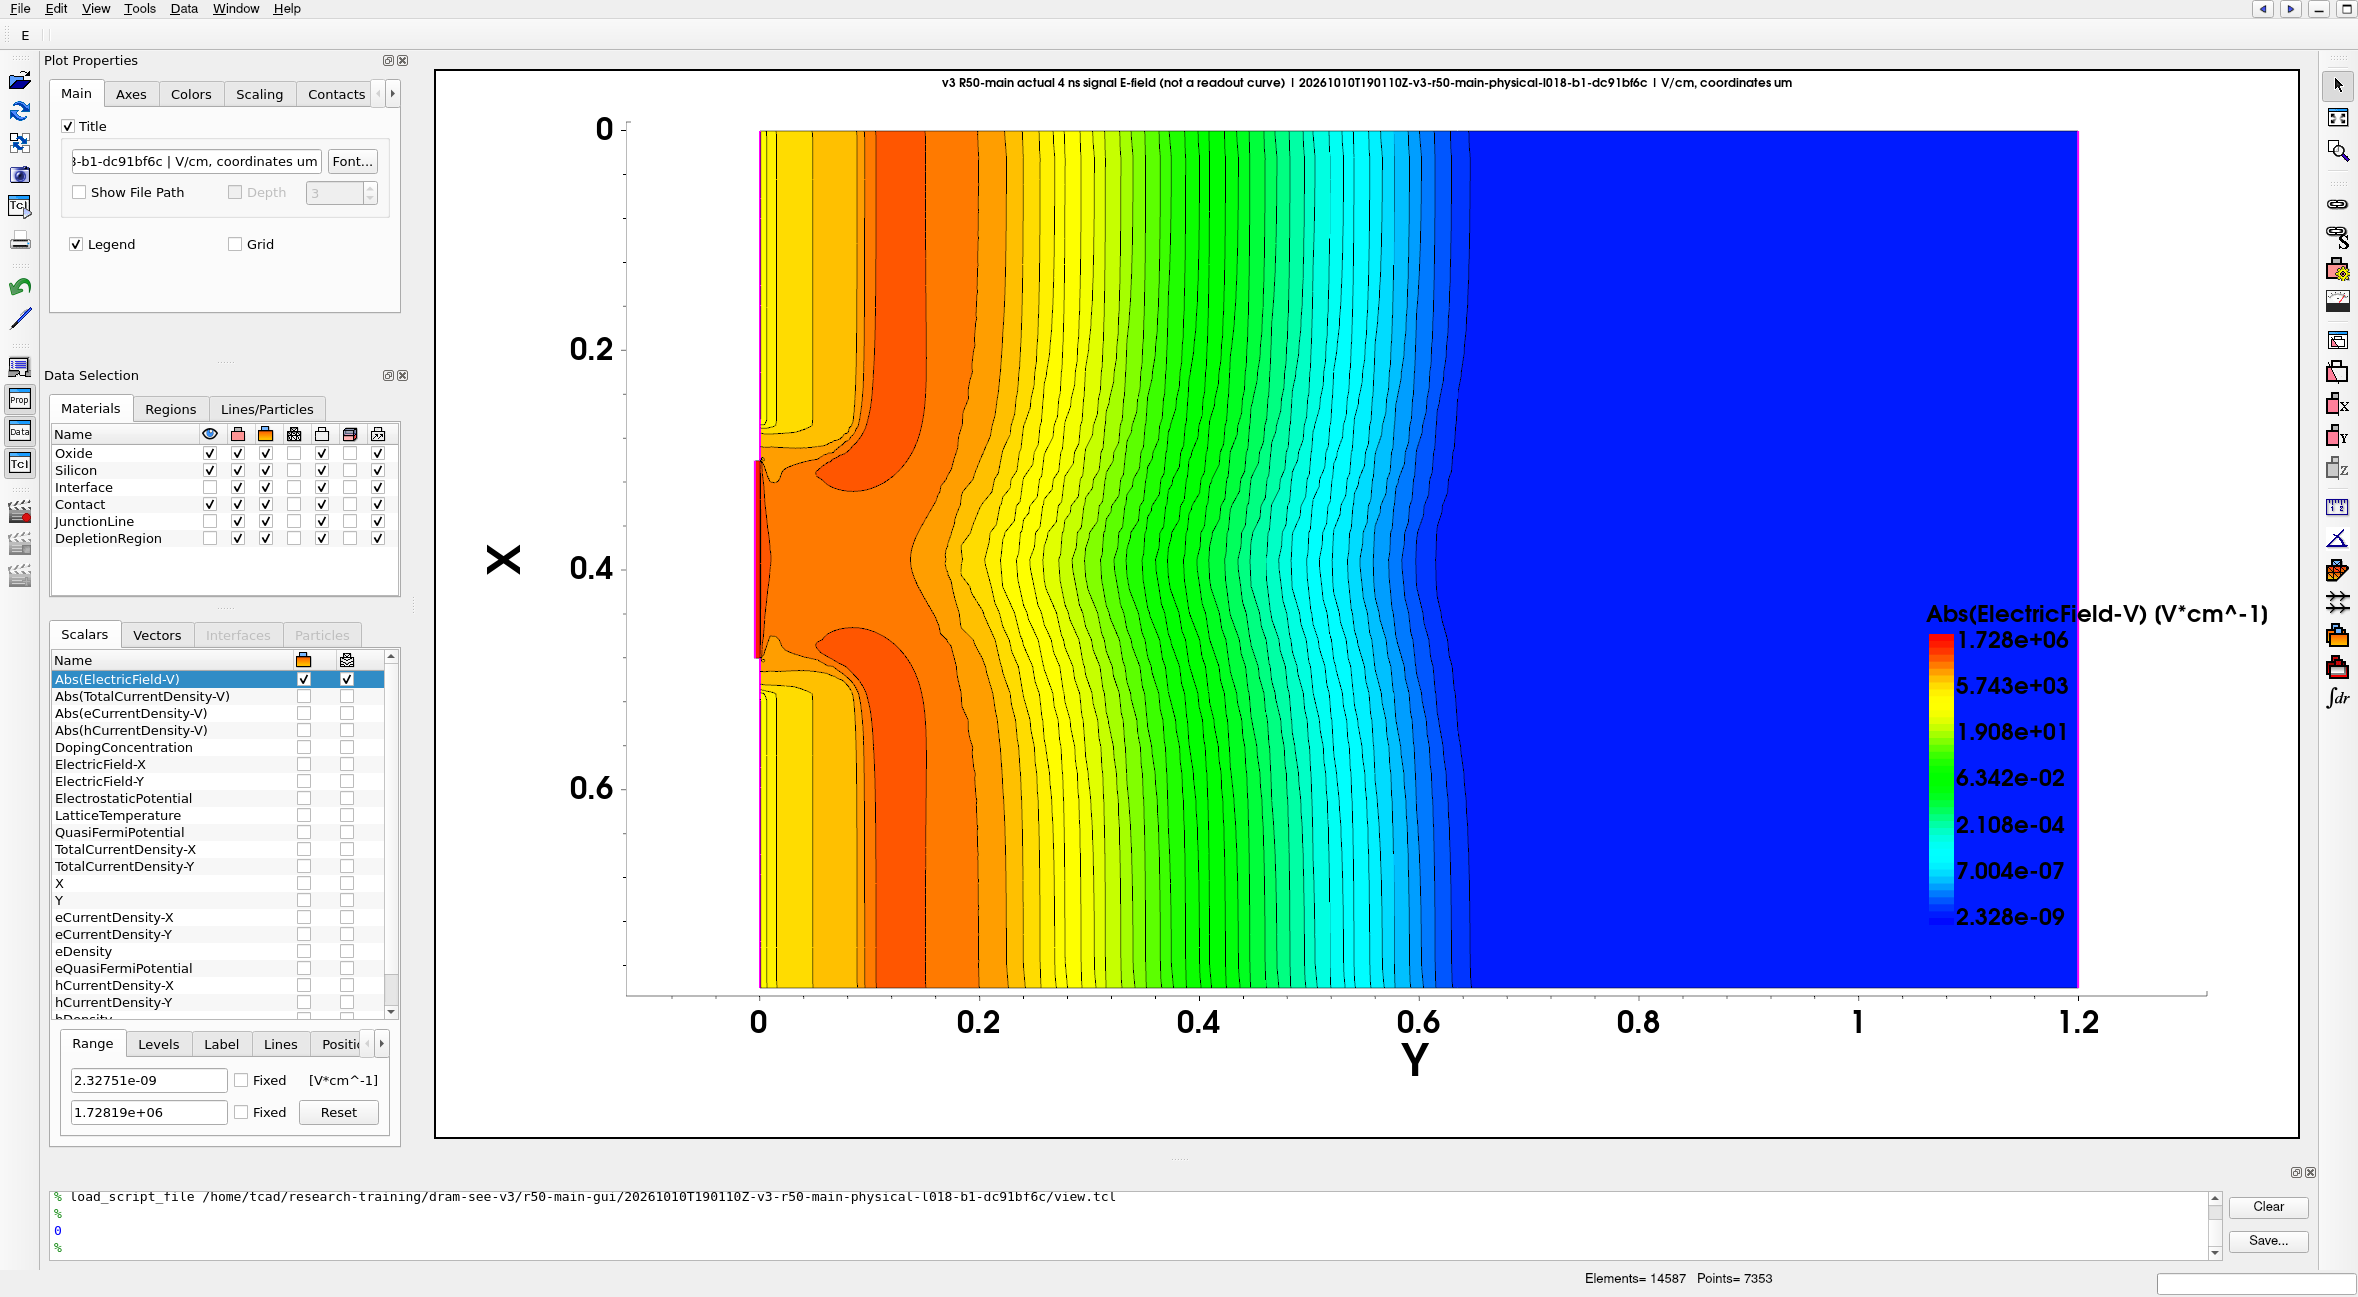
\includegraphics[width=.95\textwidth]{native-physical-window.png}
\caption{真实SVisual owned窗口：0.18~$\mu$m存储1物理参考，4~ns，Abs(ElectricField-V)，V/cm。完整窗口原字节保留并经主代理逐图目视。}
\label{cr:nativephysical}
\end{figure}

\begin{figure}[htbp]
\centering
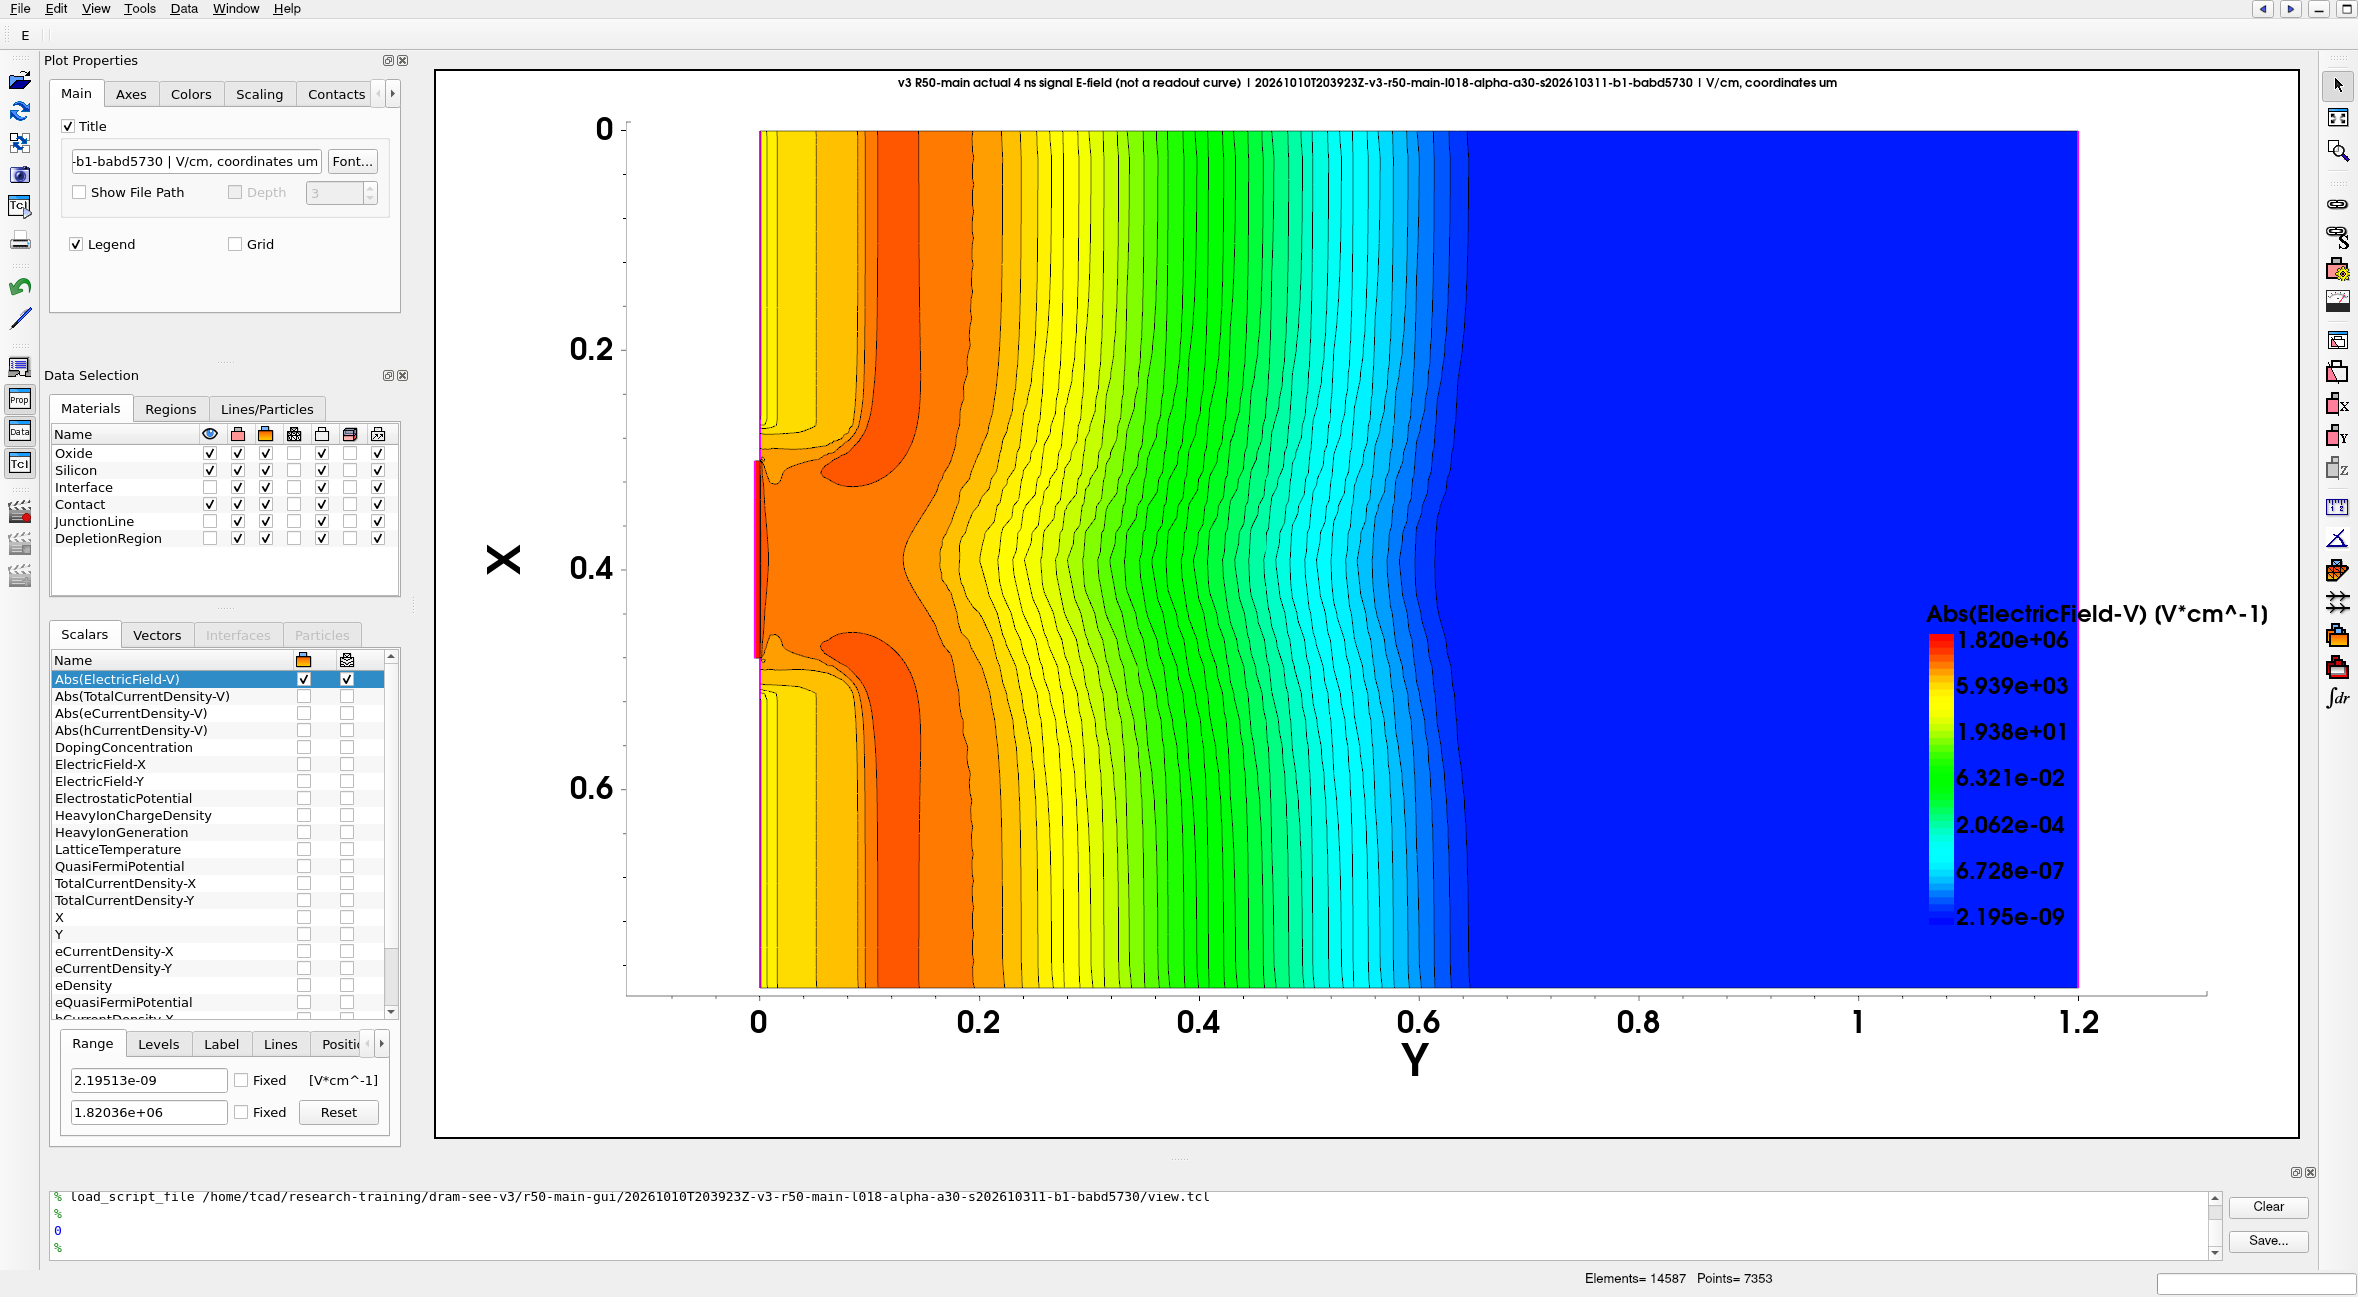
\includegraphics[width=.95\textwidth]{native-event-window.png}
\caption{真实SVisual owned窗口：0.18~$\mu$m、alpha、30°、seed202610311、bit1，4~ns。所示为原窗口，不是数据后处理绘图。}
\label{cr:nativeevent}
\end{figure}
对应1400×1000原生导出右端图例单位后缀存在裁切，已保留并如实记录；本文只展示同组完整owned窗口。真实窗口证明声明的run/变量/时刻，不证明通过Workbench Run按钮调度。
\subsection{失败保全与完整费用}

\begin{table}[htbp]
\centering\small
\caption{四个主线原始工程FAILED及其有效alias。null表示原始退出码未观测，不补写为0。}
\label{cr:failures}
\begin{tabular}{llll}
\toprule
原seed/位 & 有效重试版本 & 原状态 & 原runner退出码\\
\midrule
202610394-b1 & retry-r2 & FAILED & null（未观测）\\
202610353-b0 & retry-r3 & FAILED & null（未观测）\\
202610361-b0 & retry-r3 & FAILED & null（未观测）\\
202610371-b1 & retry-r4 & FAILED & null（未观测）\\
\bottomrule
\end{tabular}

\end{table}
完整历史账本共有7条FAILED记录；表中四项仅是R50主矩阵对应的确定性重试别名。最终逻辑槽失败为0，不表示历史失败为0，全部7条仍在原账本和快照中保留。
唯一全局账本已结算100022.07~s，约27.784~h；含原版本、probe、失败、重试与扩展。当前授权无上限，未结0项、费用缺项0项。该累计求解成本不是学生投入时长或AI效率对照。
\FloatBarrier
